\chapter{Asymptotic Safety of Gravity-Matter Systems}
\blindtext
\section{Matter contributions}
\begin{align}
	\Gammak = \Gamma_{\text{EH}} + \mathcal{S}_{\text{gf}}+ \mathcal{S}_{\text{gh}}+ \Gamma_{\text{matter}}
\end{align}
where the different matter contributions come from
\begin{align}
	\Gamma_{\text{matter}} = \mathcal{S}_{\text{S}} + \mathcal{S}_{\text{D}} + \mathcal{S}_{\text{V}} 
\end{align}
with 
\begin{align}
	\mathcal{S}_{\text{S}} &= \frac{Z_{\text{S}}}{2}\int_x \sqrt{\operatorname{det}g} \ g^{\mu\nu} \ \sum\limits_{i=1}^{N_{\text{S}}} \partial_{\mu}\phi^{i}\partial_{\nu}\phi^{i} \\
	\phantom{.}\nonumber\\
	\mathcal{S}_{\text{D}} &= iZ_{\text{D}}\int_x \sqrt{\operatorname{det}g} \ \sum\limits_{i=1}^{N_{\text{D}}} \bar{\psi}^{i}\slashed{\nabla}\psi^{i}\\
	\phantom{.}\nonumber\\
		\mathcal{S}_{\text{V}} &= \frac{Z_{\text{V}}}{4}\int_x \sqrt{\operatorname{det}g} \ \sum\limits_{i=1}^{N_{\text{V}}} g^{\mu\nu}g^{\kappa\lambda}F^{i}_{\mu\kappa}F^{i}_{\nu\lambda} \nonumber \\
		&+ \frac{Z_{\text{V}}}{2\xi}\int_x \sqrt{\operatorname{det}\bar{g}} \ \sum\limits_{i=1}^{N_{\text{V}}} \left(\bar{g}^{\mu\nu}\bar{D}_{\mu}A_{\nu}^{i}\right)^2  \\
		&+ \frac{1}{2}\int_x \sqrt{\operatorname{det}\bar{g}} \ \sum\limits_{i=1}^{N_{\text{V}}} \bar{c}_i(-\bar{D}^2)c_i \nonumber
\end{align}
Covariant derivative:
\begin{align}
	\nabla_{\mu} = \partial_{\mu} + \frac{1}{8}\left[\gamma^{a}, \gamma^{b}\right]\omega_{\mu}^{ab}
\end{align}
\blindtext
 \begin{figure}[H]
 \centering
 \hfill
 \begin{subfigure}{0.3\textwidth} 
	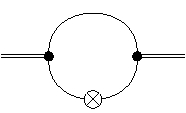
\includegraphics[width=\textwidth]{figs/TikZ/fermion_contribution}
 	\subcaption{Fermions.}
 \end{subfigure}
 \hfill
 \begin{subfigure}{0.3\textwidth} 
 	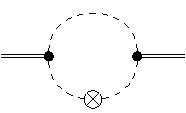
\includegraphics[width=\textwidth]{figs/TikZ/scalar_contribution}
 	\subcaption{Scalars.}
 \end{subfigure} 
 \hfill
 \begin{subfigure}{0.3\textwidth} 
 	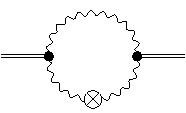
\includegraphics[width=\textwidth]{figs/TikZ/gauge_field_contribution}
 	\subcaption{Gauge Fields.}
 \end{subfigure} 
 \hfill
 \caption{Different matter contributions to the graviton anomalous dimension $\eta_h$.}	
 \end{figure}
 
 \blindtext
 
  \begin{figure}[H]
 \centering
 \hfill
 \begin{subfigure}{0.3\textwidth} 
	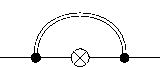
\includegraphics[width=\textwidth]{figs/TikZ/graviton_fluctuations1}
 \end{subfigure}
 \hfill
 \begin{subfigure}{0.3\textwidth}
 \vspace{-3.5pt}
 	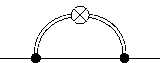
\includegraphics[width=\textwidth]{figs/TikZ/graviton_fluctuations2}
 \end{subfigure} 
 \hfill
 \begin{subfigure}{0.3\textwidth} 
 	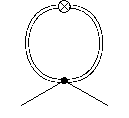
\includegraphics[scale = 1.5]{figs/TikZ/graviton_fluctuations3}
 \end{subfigure} 
 \hfill
 \caption{Contributing diagrams to the fermion anomalous dimension $\eta_D$. Analogous contributions arise for external scalars and gauge fields to $\eta_S$ and $\eta_V$.} 	
 \end{figure}